\subsubsection{Implement network security}

\textbf{Azure Virtual Network} \\
Design best practices:
\begin{enumerate}
\item Minimise conflicts. \textit{Ensure non-overlapping address spaces. The VNet address space (CIDR block) should not overlap with your organization's other network ranges.}
\item Keep a reserve space. \textit{Reserve some of the address space of the VNet.}
\item Minimise management overhead. \textit{Create a few large VNets, rather than multiple small VNets.}
\item Secure it. \textit{Secure your VNet using Network Security Groups (NSGs)}.
\end{enumerate}

Communication: \\
All resources in a VNet can communicate outbound to the internet, by default. You can communicate inbound to a resource by assigning a public IP address or a public Load Balancer. When using only an internal Standard Load Balancer, outbound connectivity is not available until you define how you want outbound connections to work with an instance-level public IP or a public Load Balancer.

The communication options of Azure resources are:
\begin{itemize}
\item Virtual network: \textit{Deploy VMs, and other Azure resources to a virtual network, such as Azure App Service Environments, the Azure Kubernetes Service (AKS), or Azure Virtual Machine Scale Sets.}
\item Through a virtual network service endpoint: \textit{Extend your virtual network private address space and the identity of your virtual network to Azure service resources, such as Azure Storage accounts and Azure SQL databases, over a direct connection. Service endpoints allow you to secure your critical Azure service resources to only a virtual network.}
\item VNet Peering: \textit{Connect virtual networks to each other, enabling resources in either virtual network to communicate with each other, using virtual network peering. The virtual networks you connect can be in the same, or different, Azure regions.}
\end{itemize}

The communication options for on-premise resources are:
\begin{itemize}
\item Point-to-site virtual private network (VPN): \textit{Established between a virtual network and a single computer in your network. Each computer must configure an individual connection. Intended for developers, as it requires few adjustments to existing network. The communication is encrypted.}
\item Site-to-site VPN: \textit{Established between on-premises VPN device and an Azure VPN Gateway in a virtual network. This connection type enables any on-premises resource that you authorize to access a virtual network. The communication is encrypted.}
\item Azure ExpressRoute: \textit{Established between your network and Azure, through an ExpressRoute partner. This connection is private. Traffic does not go over the internet.}
\end{itemize}

You can filter network traffic between subnets using either or both of the following options:
\begin{itemize}
\item Security groups: \textit{Network security groups and application security groups can contain multiple inbound and outbound security rules that enable you to filter traffic to and from resources by source and destination IP address, port, and protocol.}
\item Network virtual appliances:\textit{A network virtual appliance is a VM that performs a network function, such as a firewall, WAN optimization, or other network function.}
\end{itemize}

Azure routes traffic between subnets, connected virtual networks, on-premises networks, and the Internet, by default. You can implement either or both of the following options to override the default routes Azure creates:
\begin{itemize}
\item Route tables: \textit{Custom route tables with routes that control where traffic is routed to for each subnet.}
\item Border gateway protocol (BGP) routes: \textit{Connect the virtual network to the on-premises network using an Azure VPN Gateway or ExpressRoute connection, you can propagate your on-premises BGP routes to your virtual networks. }
\end{itemize}

\textbf{Network Security Groups} \\
Security rules in network security groups enable you to filter the type of network traffic that can flow in and out of virtual network subnets and network interfaces.

A network security group (NSG) contains a list of security rules that allow or deny network traffic to resources connected to Azure Virtual Networks (VNet). NSGs can be associated to subnets, individual VMs (classic), or individual network interfaces (NIC) attached to VMs (Resource Manager).  When an NSG is associated to a subnet, the rules apply to all resources connected to the subnet. Traffic can further be restricted by also associating an NSG to a VM or NIC.

\begin{figure}[!h]
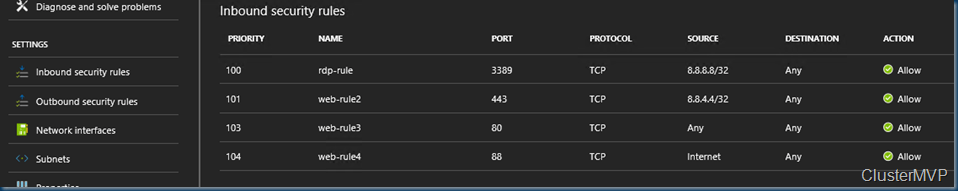
\includegraphics[width=1\textwidth]{platform-network-rules.png}
\caption{List of inbound security rules}
\end{figure}


\textbf{Application Security Groups} \\
Feature for security micro-segmentation for your virtual networks in Azure.
\begin{figure}[!h]
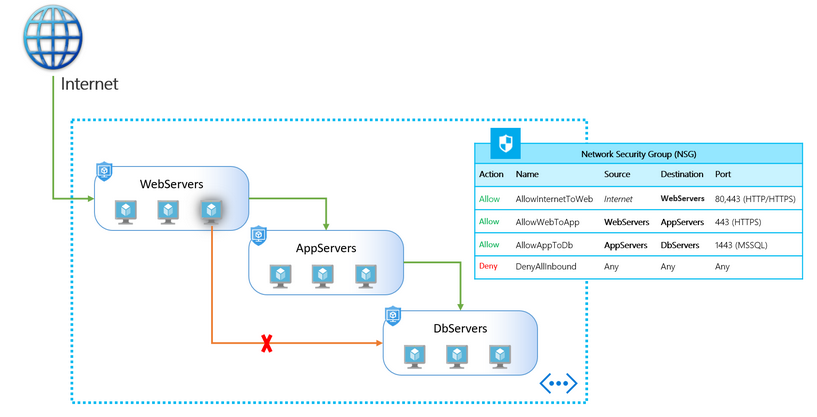
\includegraphics[width=1\textwidth]{platform-network-application-security-groups.png}
\caption{Application Security Groups (ASG) in all Azure regions}
\end{figure}

\underline{Network segmentation.} Centralized on applications, instead of explicit IP addresses. Implementing granular security traffic controls improves isolation of workloads and protects them individually. 

Filtering traffic based on applications patterns
\begin{itemize}
\item Define your application groups
\item Define a single collection of rules using ASGs and Network Security Groups (NSG)
\item Scale at your own pace. When you deploy VMs, make them members of the appropriate ASGs. \textit{Implement a zero-trust model, limiting access to the application flows that are explicitly permitted.}
\end{itemize}

\textbf{Firewall} \\
Outbound network access controls:
\begin{itemize}
\item Application rules that define fully qualified domain names (FQDNs) that can be accessed from a subnet.
\item Network rules that define source address, protocol, destination port, and destination address.
\end{itemize}

\subsubsection{Security management}
For more secure management and operations, you can minimize a client’s attack surface by reducing the number of possible entry points. This can be done through security principles: “separation of duties” and “segregation of environments.”

\begin{itemize}
\item Isolate sensitive functions \textit{from one another to decrease the likelihood that a mistake at one level leads to a breach in another. I.e. do not perform tasks such as browsing or email on secured workstations.}
\item Reduce the system’s attack surface by removing unnecessary software \textit{i.e. email client and productivity applications.}
\item Secure management workstations. \textit{Client systems that have administrator access to infrastructure components should be subjected to the strictest possible policy to reduce security risks.}
	\begin{itemize}
	\item Security policies > Group Policy > Deny open Internet access
	\item Use Internet Protocol security (IPsec) VPNs if direct access is needed
	\item Separate management and development Active Directory domains
	\item Isolate and filter management workstation network traffic
	\item Antimalware software
	\item Multi-factor authentication 
	\end{itemize}
\end{itemize}

\textbf{Security mechanisms}\\
Azure provides security mechanisms to aid administrators who manage Azure cloud services and virtual machines. These mechanisms include:

\begin{itemize}
\item Authentication and role-based access control.
\item Monitoring, logging, and auditing.
\item Certificates and encrypted communications.
\item A web management portal.
\item Network packet filtering.
\end{itemize}

\textbf{Hardened workstation}
\begin{itemize}
\item Active scanning and patching.
\item Limited functionality.
\item Network hardening. \textit{Use Windows Firewall rules to allow only valid IP addresses, ports, and URLs related to Azure management. Ensure that inbound remote connections to the workstation are also blocked.}
\item Execution restriction. \textit{Allow only a set of predefined executable files that are needed for management to run (referred to as “default-deny”).}
\item Least privilege. \textit{Management workstation users should not have any administrative privileges on the local machine itself. }
\end{itemize}
You can enforce all this by using Group Policy Objects (GPOs) in Active Directory Domain Services (AD DS) and applying them through your (local) management domain to all management accounts.

\begin{itemize}
\item IE hardening. \textit{Review your client policies and enforce running in protected mode, disabling add-ons, disabling file downloads, and using Microsoft SmartScreen filtering. Ensure that security warnings are displayed. Take advantage of Internet zones and create a list of trusted sites for which you have configured reasonable hardening. Block all other sites and in-browser code, such as ActiveX and Java.}
\item Standard user. \textit{Running as a standard user brings a number of benefits, the biggest of which is that stealing administrator credentials via malware becomes more difficult. In addition, a standard user account does not have elevated privileges on the root operating system, and many configuration options and APIs are locked out by default.}
\item AppLocker. \textit{Use AppLocker to restrict the programs and scripts that users can run. You can run AppLocker in audit or enforcement mode. By default, AppLocker has an allow rule that enables users who have an admin token to run all code on the client.}
\item Code signing. \textit{Code signing all tools and scripts used by administrators provides a manageable mechanism for deploying application lockdown policies. Hashes do not scale with rapid changes to the code, and file paths do not provide a high level of security. You should combine AppLocker rules with a PowerShell execution policy that only allows specific signed code and scripts to be executed.}
\item Group Policy. \textit{Create a global administrative policy that is applied to any domain workstation that is used for management (and block access from all others), and to user accounts authenticated on those workstations.}
\item Security-enhanced provisioning. \textit{Safeguard your baseline hardened workstation image to help protect against tampering. Use security measures like encryption and isolation to store images, virtual machines, and scripts, and restrict access (consider using an auditable check-in/check-out process).}
\item Patching. 
\item Encryption. \textit{Make sure that management workstations have a Trusted Platform Module}
\item Governance. Use \textit{AD DS GPOs to control all the administrators’ Windows interfaces, such as file sharing. Include management workstations in auditing, monitoring, and logging processes. Track all administrator and developer access and usage.}
\end{itemize}

\textbf{Best practices} \\
\begin{tabular}{p{7.3cm} p{7.3cm}}
\textbf{Do} & \textbf{Don't} \\
\hline 
Maintain confidentiality by delivering account names and passwords directly, perform a remote installation of client/server certificates (via an encrypted session), download from a protected network share, or distribute by hand via removable media. & Don't email credentials for administrator access or other secrets (for example, SSL or management certificates) \\
\hline 
Proactively manage certificate life cycles. &  \\
\hline 
Establish security management principles and system hardening policies. Apply them to your development environments. & Don't store account passwords unencrypted or un-hashed. \\
\hline 
Use Enhanced Mitigation Experience Toolkit 5.5 certificate pinning rules to ensure proper access to Azure SSL/TLS sites. &  \\
\hline 
Create a dedicated Microsoft account to manage your Azure subscription & Don't share accounts and passwords between administrators, or reuse passwords across multiple user accounts or services, particularly those for social media or other non-administrative activities. \\
\hline
Configuration files and profiles should be installed from a trusted source. & Don't email configuration files. \\
\hline
Enforce strong password policies, expiration cycles (changeon-first-use), console timeouts, and automatic account lockouts. Use a client password management system with multi-factor authentication for password vault access. & Don't use weak or simple logon passwords. \\
\hline
Lock down Azure ports and IP addresses to restrict management access. & Don't expose management ports to the Internet. \\
\hline
Use firewalls, VPNs, and NAP for all management connections.
\end{tabular}

\clearpage
\textbf{Azure Storage firewalls} \\
Azure Storage provides a layered security model. This model enables you to secure and control the level of access to your storage accounts that your applications and enterprise environments demand, based on the type and subset of networks used. When network rules are configured, only applications requesting data over the specified set of networks can access a storage account. You can limit access to your storage account to requests originating from specified IP addresses, IP ranges or from a list of subnets in an Azure Virtual Network (VNet).

An application that accesses a storage account when network rules are in effect still requires proper authorization for the request. Authorization is supported with Azure Active Directory (Azure AD) credentials for blobs and queues, with a valid account access key, or with an SAS token.

Turning on firewall rules for your storage account blocks incoming requests for data by default, unless the requests originate from a service operating within an Azure Virtual Network (VNet) or from allowed public IP addresses. Requests that are blocked include those from other Azure services, from the Azure portal, from logging and metrics services, and so on.

You can grant access to Azure services that operate from within a VNet by allowing traffic from the subnet hosting the service instance. You can also enable a limited number of scenarios through the Exceptions mechanism.

\begin{tabular}{c c p{6cm}}

\end{tabular}